%% the_assembly.tex
%% Author: Leighton Pritchard
%% Copyright: James Hutton Institute
%% These slides give a short account of what you can 
%% expect back from sequence assembly

% SUBSECTION: What you get back
% What you get back from assembly
\subsection{What you get back}

% What you get back in an ideal world
\begin{frame}
  \frametitle{In an ideal world}
  Ideally, you would have one sequence per chromosome/plasmid.\\
  (and no errors): a \textbf{closed/complete} genome.
  \begin{center}
    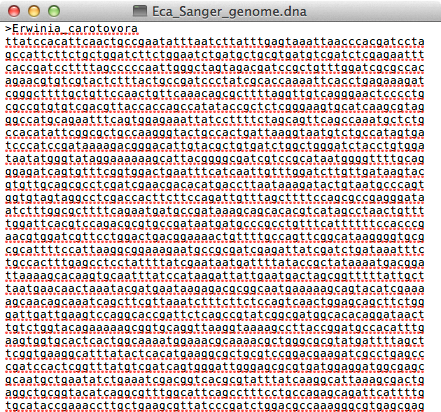
\includegraphics[width=0.5\textwidth]{images/pba_sequence}
    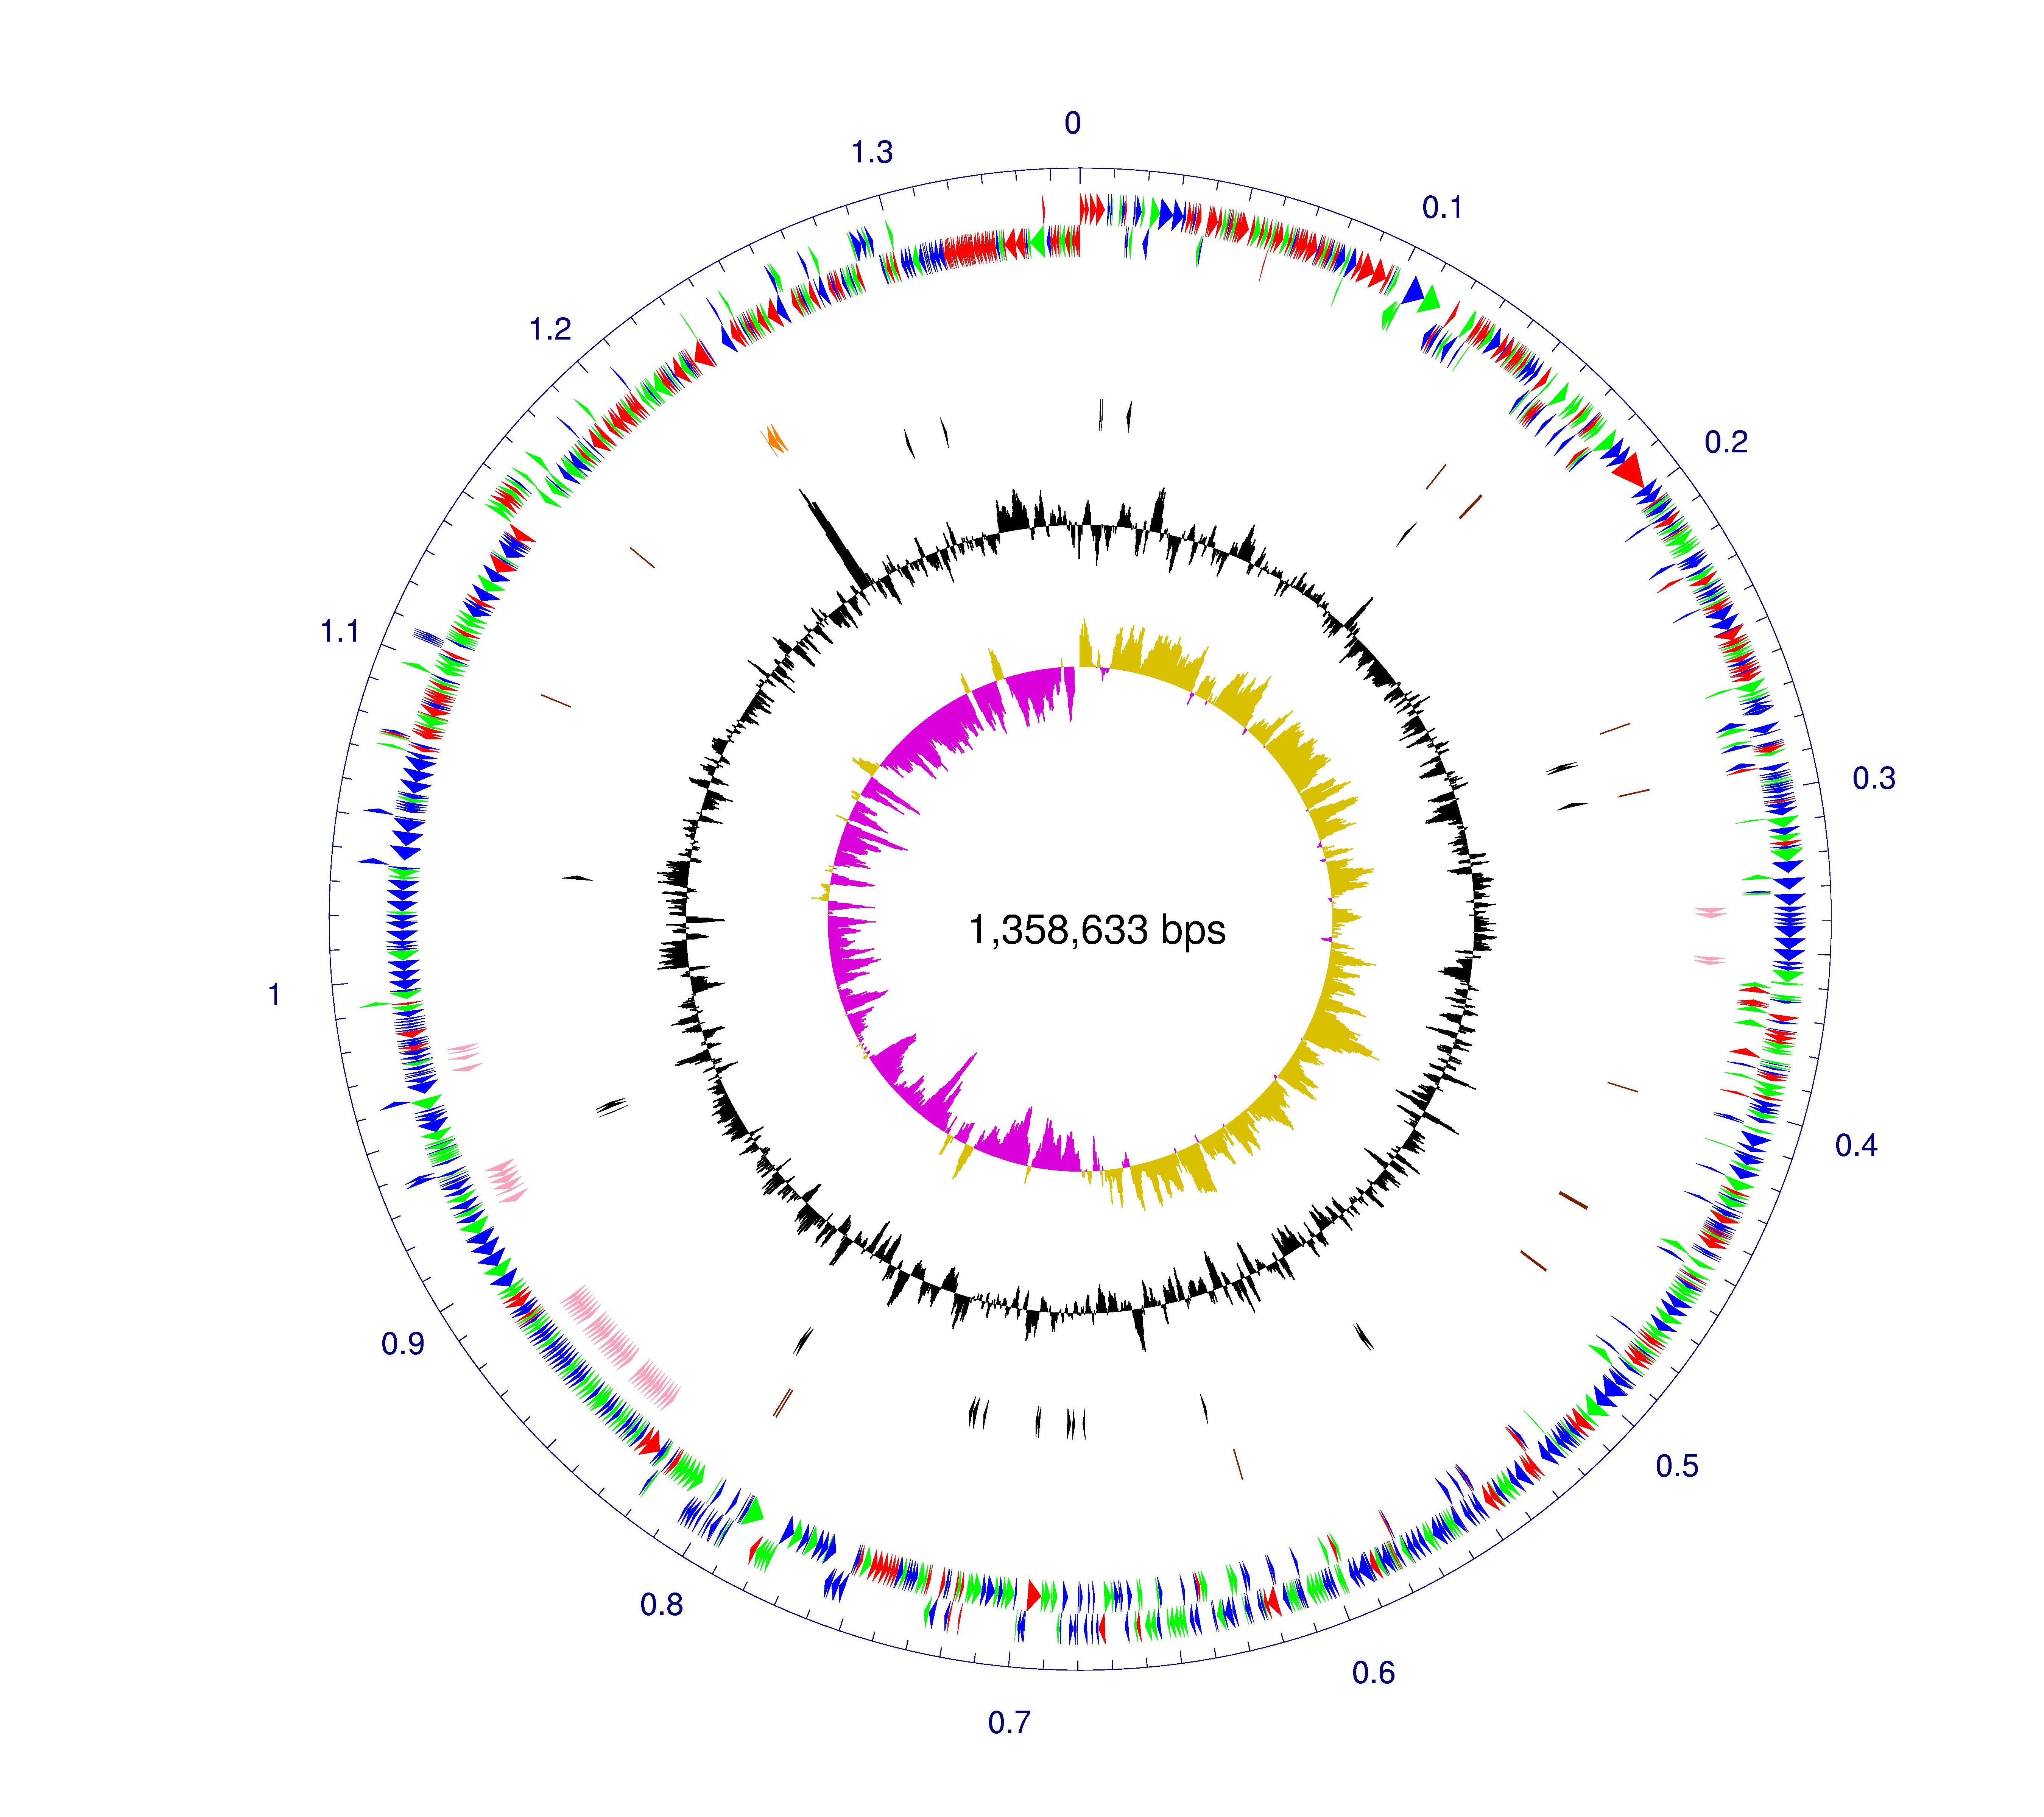
\includegraphics[width=0.5\textwidth]{images/complete_genome_circle}
  \end{center}    
  PacBio, Sanger, manual closing, Nanopore(?)
\end{frame}

% What you get back in an ideal world
\begin{frame}
  \frametitle{More realistically$\ldots$}
  Typically, a number of assembled fragments (contigs or scaffold) are returned in FASTA format: a \textbf{draft}, \textit{disordered} genome.\\
  Around 250 contigs for a 5Mbp genome is usual with Illumina\\
  \begin{center}
    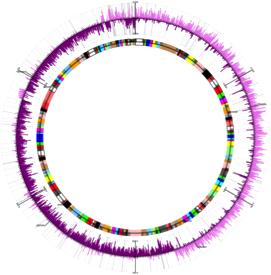
\includegraphics[width=0.5\textwidth]{images/circle_1}
    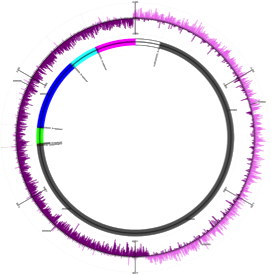
\includegraphics[width=0.5\textwidth]{images/circle_3}
  \end{center}    
\end{frame}

% Ordering fragments
\begin{frame}
  \frametitle{Ordering contigs}
  Contigs can be ordered correctly into \textit{scaffolds} if paired-end reads span gaps (typically done during assembly).\\
  Gaps are usually filled with \texttt{N}s (length estimated)
  \begin{center}
    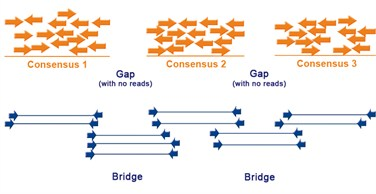
\includegraphics[width=1\textwidth]{images/contig_order_pe}
  \end{center}    
\end{frame}

% Ordering fragments
\begin{frame}
  \frametitle{Ordering contigs}
  Contigs and scaffolds can also be reordered by alignment to a reference genome.\\
  \begin{itemize}
    \item Mauve/progressiveMauve\footnote{\tiny{\href{http://dx.doi.org/10.1101/gr.2289704}{Darling \textit{et al}. (2004) \textit{Genome Res.} \textbf{14}:1394-1403 doi:10.1101/gr.2289704}}}
    \item MUMmer\footnote{\tiny{\href{http://dx.doi.org/10.1186/gb-2004-5-2-r12}{Kurtz \textit{et al}. (2004) \textit{Genome Biol.} \textbf{5}:R12 doi:10.1186/gb-2004-5-2-r12}}}
  \end{itemize}
  \begin{center}
    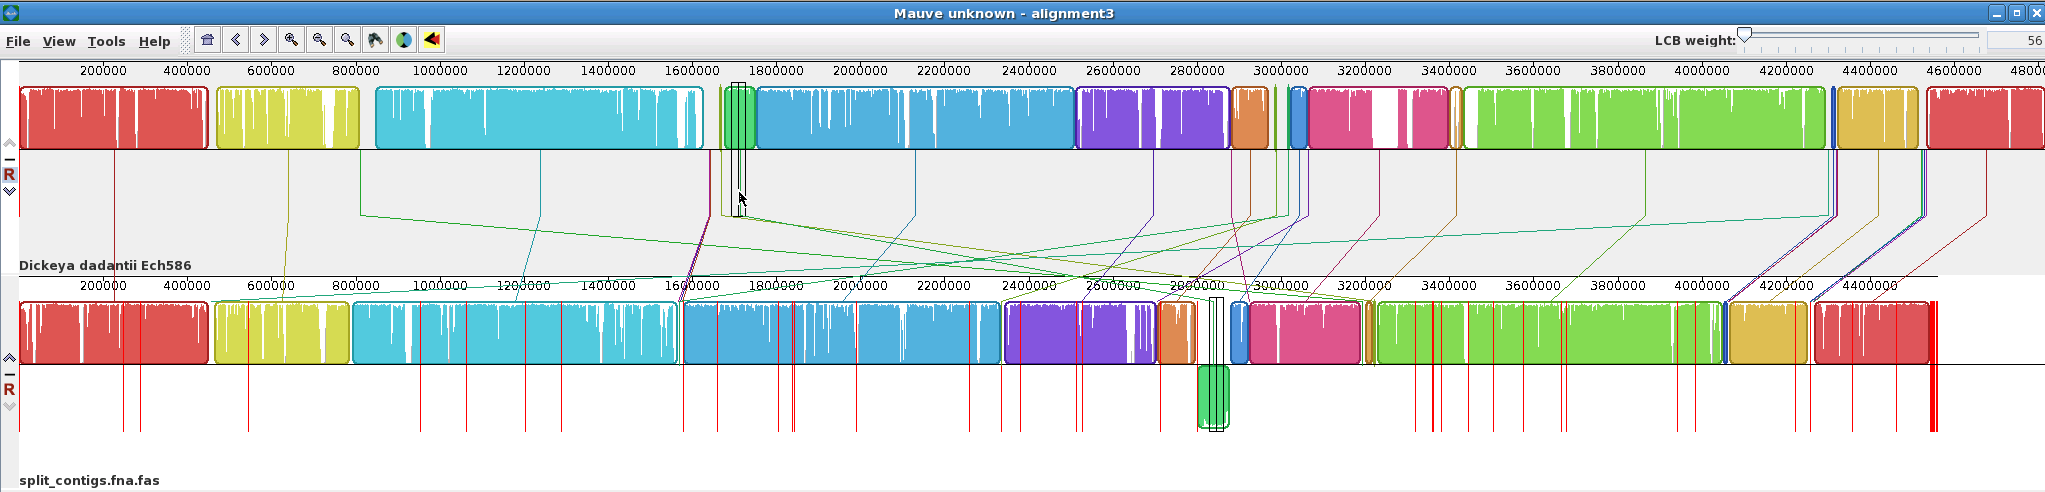
\includegraphics[width=1\textwidth]{images/mauve_output}
  \end{center}    
\end{frame}

% Ordering fragments
\begin{frame}
  \frametitle{Where next?\footnote{\tiny{\href{http://dx.doi.org/10.1093/gbe/evq048}{Lefebure \textit{et al}. (2010) \textit{Genome Biol. Evol.} \textbf{2}:646-655 doi:10.1093/gbe/evq048}}}}
  \begin{center}
    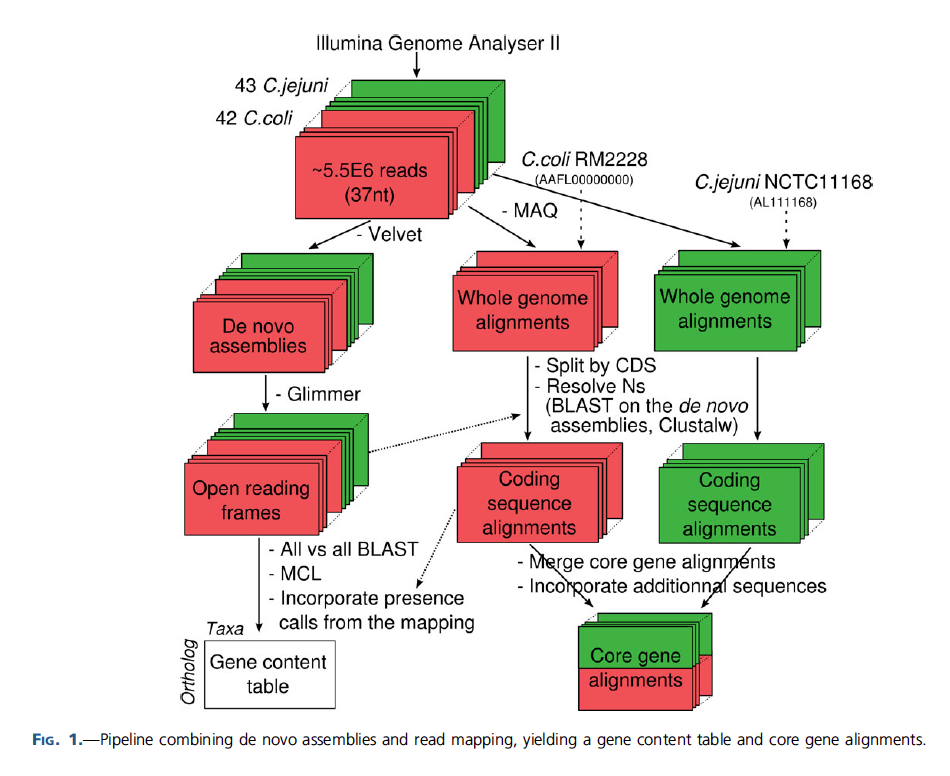
\includegraphics[width=0.8\textwidth]{images/genome_analysis_pipeline}
  \end{center}    
\end{frame}
